\documentclass[]{uc2pfecaneva}

\includepdf[pages=-]{garde.pdf}
\begin{document}
    \setlength{\parskip}{6pt}
    \tableofcontents
    \setcounter{chapter}{1}
    \chapter{Conception}
    \newpage

    \raggedright\section{Introduction}
    \clearpage


    \begin{table}
        \raggedright\section{Domain Model}
        The domain model is a visual representation of real world entities and the relationships between them, which collectively describe the problem domain space, It's used to clarify important domain-specific terms and to identify the entity classes.
        \raggedright\subsection{Entities}
        A list of all entities and brief description for each one specifying the role of that entity\linebreak \\
        \begin{tabularx}{\textwidth}{|l|X|}
            \hline
            Entity          & Description                                                                                                                                                                \\ \hline
            \textbf{User :} & the super class for all users, contains fields and methods that every user should have.\\ \hline
            \textbf{Admin :} & the admin user entity, contains admin-specific fields and methods.\\ \hline
            \textbf{Teacher :} & the class that contains all teacher types : Headteacher, AssociateTeacher and Proctor.\\ \hline
            \textbf{Student :} & the Student who pass the exam on the platform.\\ \hline
            \textbf{Question :} & contains the content of the question.\\ \hline
            \textbf{QuestionType :} & enumeration entity that holds all question types.\\ \hline
            \textbf{QuestionBank :} & contains the question list created the teachers.\\ \hline
            \textbf{Exam :} & the Exam entity, contains a question list and more.\\ \hline
            \textbf{ExamType :} & enumeration entity that holds exam types.\\ \hline
            \textbf{ExamPlanning :} & the ExamPlanning entity, contains fields about the starting date of the exam and more.\\ \hline
            \textbf{Feedback :} & the student feedback and impression after an exam session.\\ \hline
            \textbf{Group :} & Holds the name and information about a group of student assigned to an exam session.\\ \hline
            \textbf{GroupMembers :} & Holds the students list of each group.\\ \hline
            \textbf{Answer :} & the student answer of a question.\\ \hline
            \textbf{AnswerType :} & enumeration entity that holds all answer types.\\ \hline
            \textbf{Evaluation :} & the response evaluation of a question.\\ \hline
            \textbf{Correction :} & the exam correction added by the head teacher.\\ \hline
            \textbf{Module :} & the module entity, contains module-specific fields.\\ \hline
            \textbf{Teaching :} & Contains every teacher's assigned modules.\\ \hline
            \textbf{Proctoring :} & Holds the proctors list assigned to an exam session.\\ \hline
            \textbf{Comment :} & a comment of a proctor on a student in an exam session\\ \hline
            \textbf{Message :} & a message between a proctor and a student in an exam session.\\ \hline
            \textbf{Presence :} & the presence state and information of a student for an exam session.\\ \hline
            \textbf{Blocked :} & holds the students list of kicked users, so they can't join the exam session.\\ \hline
        \end{tabularx}
        \label{table:1}
    \end{table}

    \clearpage

    \begin{table}[t]
        \begin{tabularx}{\textwidth}{|l|X|}
            \hline
            \textbf{Log :} & contains exam session logs, to know the exact time each student enters or leaves the session.\\ \hline
            \textbf{Report :} & Super class for all report types.\\ \hline
            \textbf{CheatingReport :} & This class holds the information about report written by the procter when he kicks a student out of an exam session because of cheating.\\ \hline
            \textbf{BehaviorReport :} & This class holds the information about report written by the head teacher about a students inappropriate answer\\ \hline
            \textbf{Claim :} & contains the claim information when a student submits a claim about an evaluation.\\ \hline
            \textbf{ClaimResponse :} & Holds the teacher's response to a student's claim.\\ \hline
            \textbf{ClaimReportStatus :} & enumeration entity that holds status that a claim or report can have (Open, Closed,...).\\ \hline
            \textbf{Color :} & enumeration entity that holds colors used to display exams on a calendar.\\ \hline
            \textbf{Notification :} & Notification class for all user types.\\ \hline
            \textbf{NotificationStatus :} &  enumeration entity that holds status of a notification (Created, Delivered, Deleted,...).\\ \hline
            \textbf{AcademicYear :} & the Academic Year entity, contains fields and methods for the Academic Year.\\ \hline
            \textbf{Department :} & the Department entity, contains fields and methods for the Department.\\ \hline
        \end{tabularx}
        \caption{Entities Description}
        \label{table:1}
    \end{table}

    \begin{figure}
        \subsection{Domain class diagram}
        \raggedright Defines the domain classes and specifies the relations between these classes
        \linebreak
        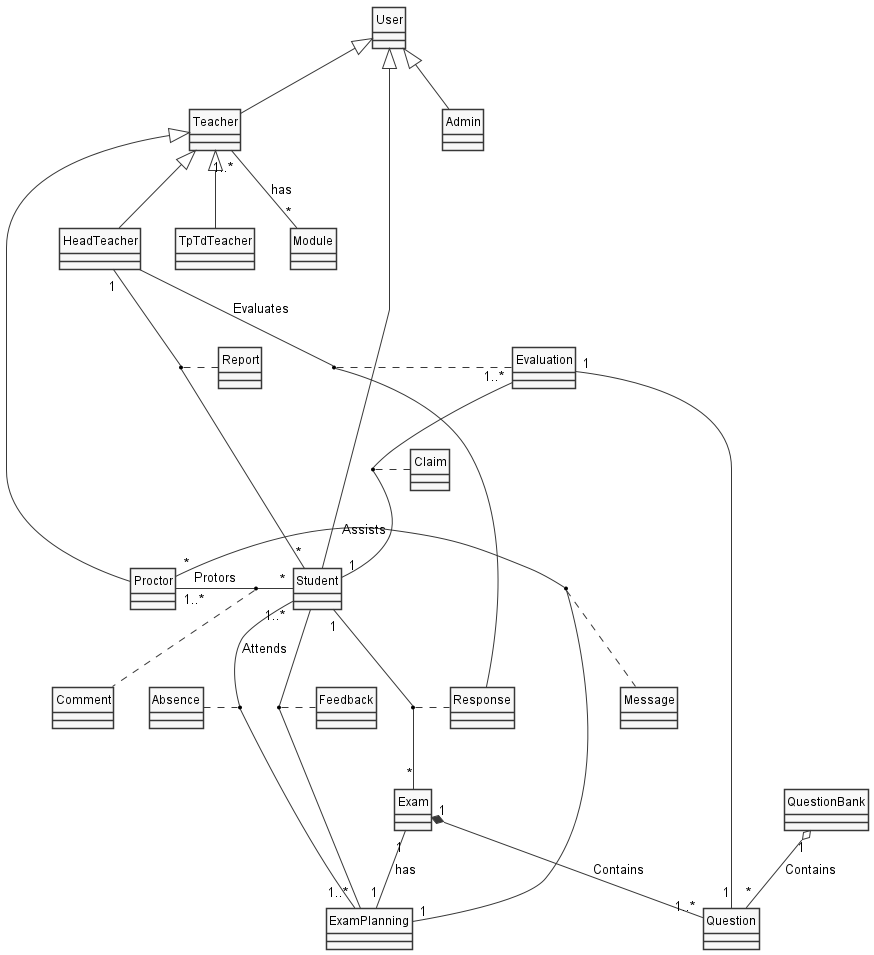
\includegraphics[width=\textwidth]{images/DCD}
        \caption{Domain class diagram}
    \end{figure}


    \begin{figure}
        \section{Conception class diagram}
        \raggedright Defines the conceptual classes with details, specifying the fields and methods of each class.
        \linebreak
        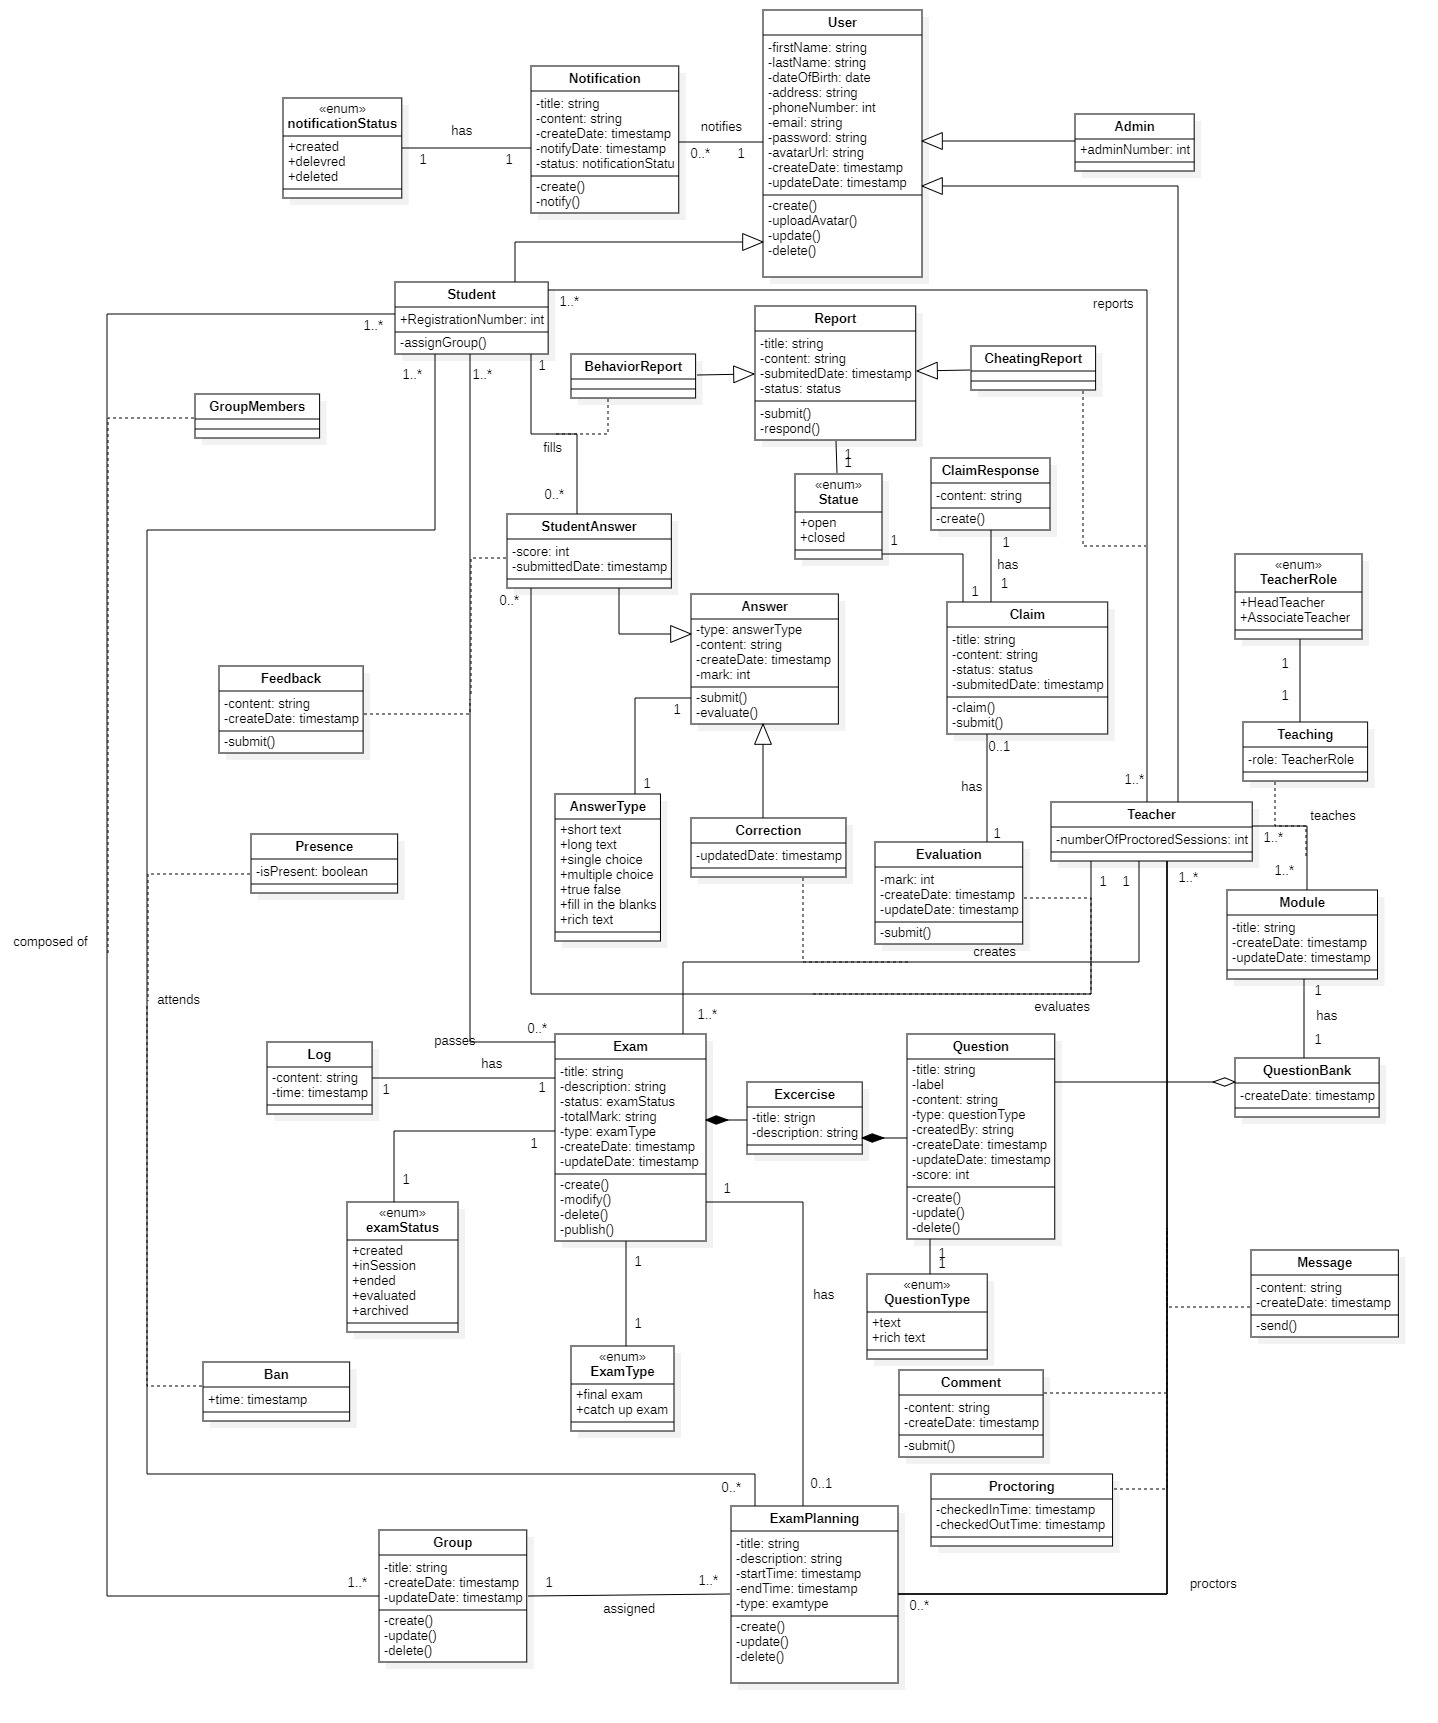
\includegraphics[width=\textwidth]{images/CCD}
        \caption{Conception class diagram}
    \end{figure}
    \clearpage

    \begin{figure}
        \raggedright\section{Migration to database}

        \raggedright Shows the database tables and their relations and attributes.
        \linebreak
        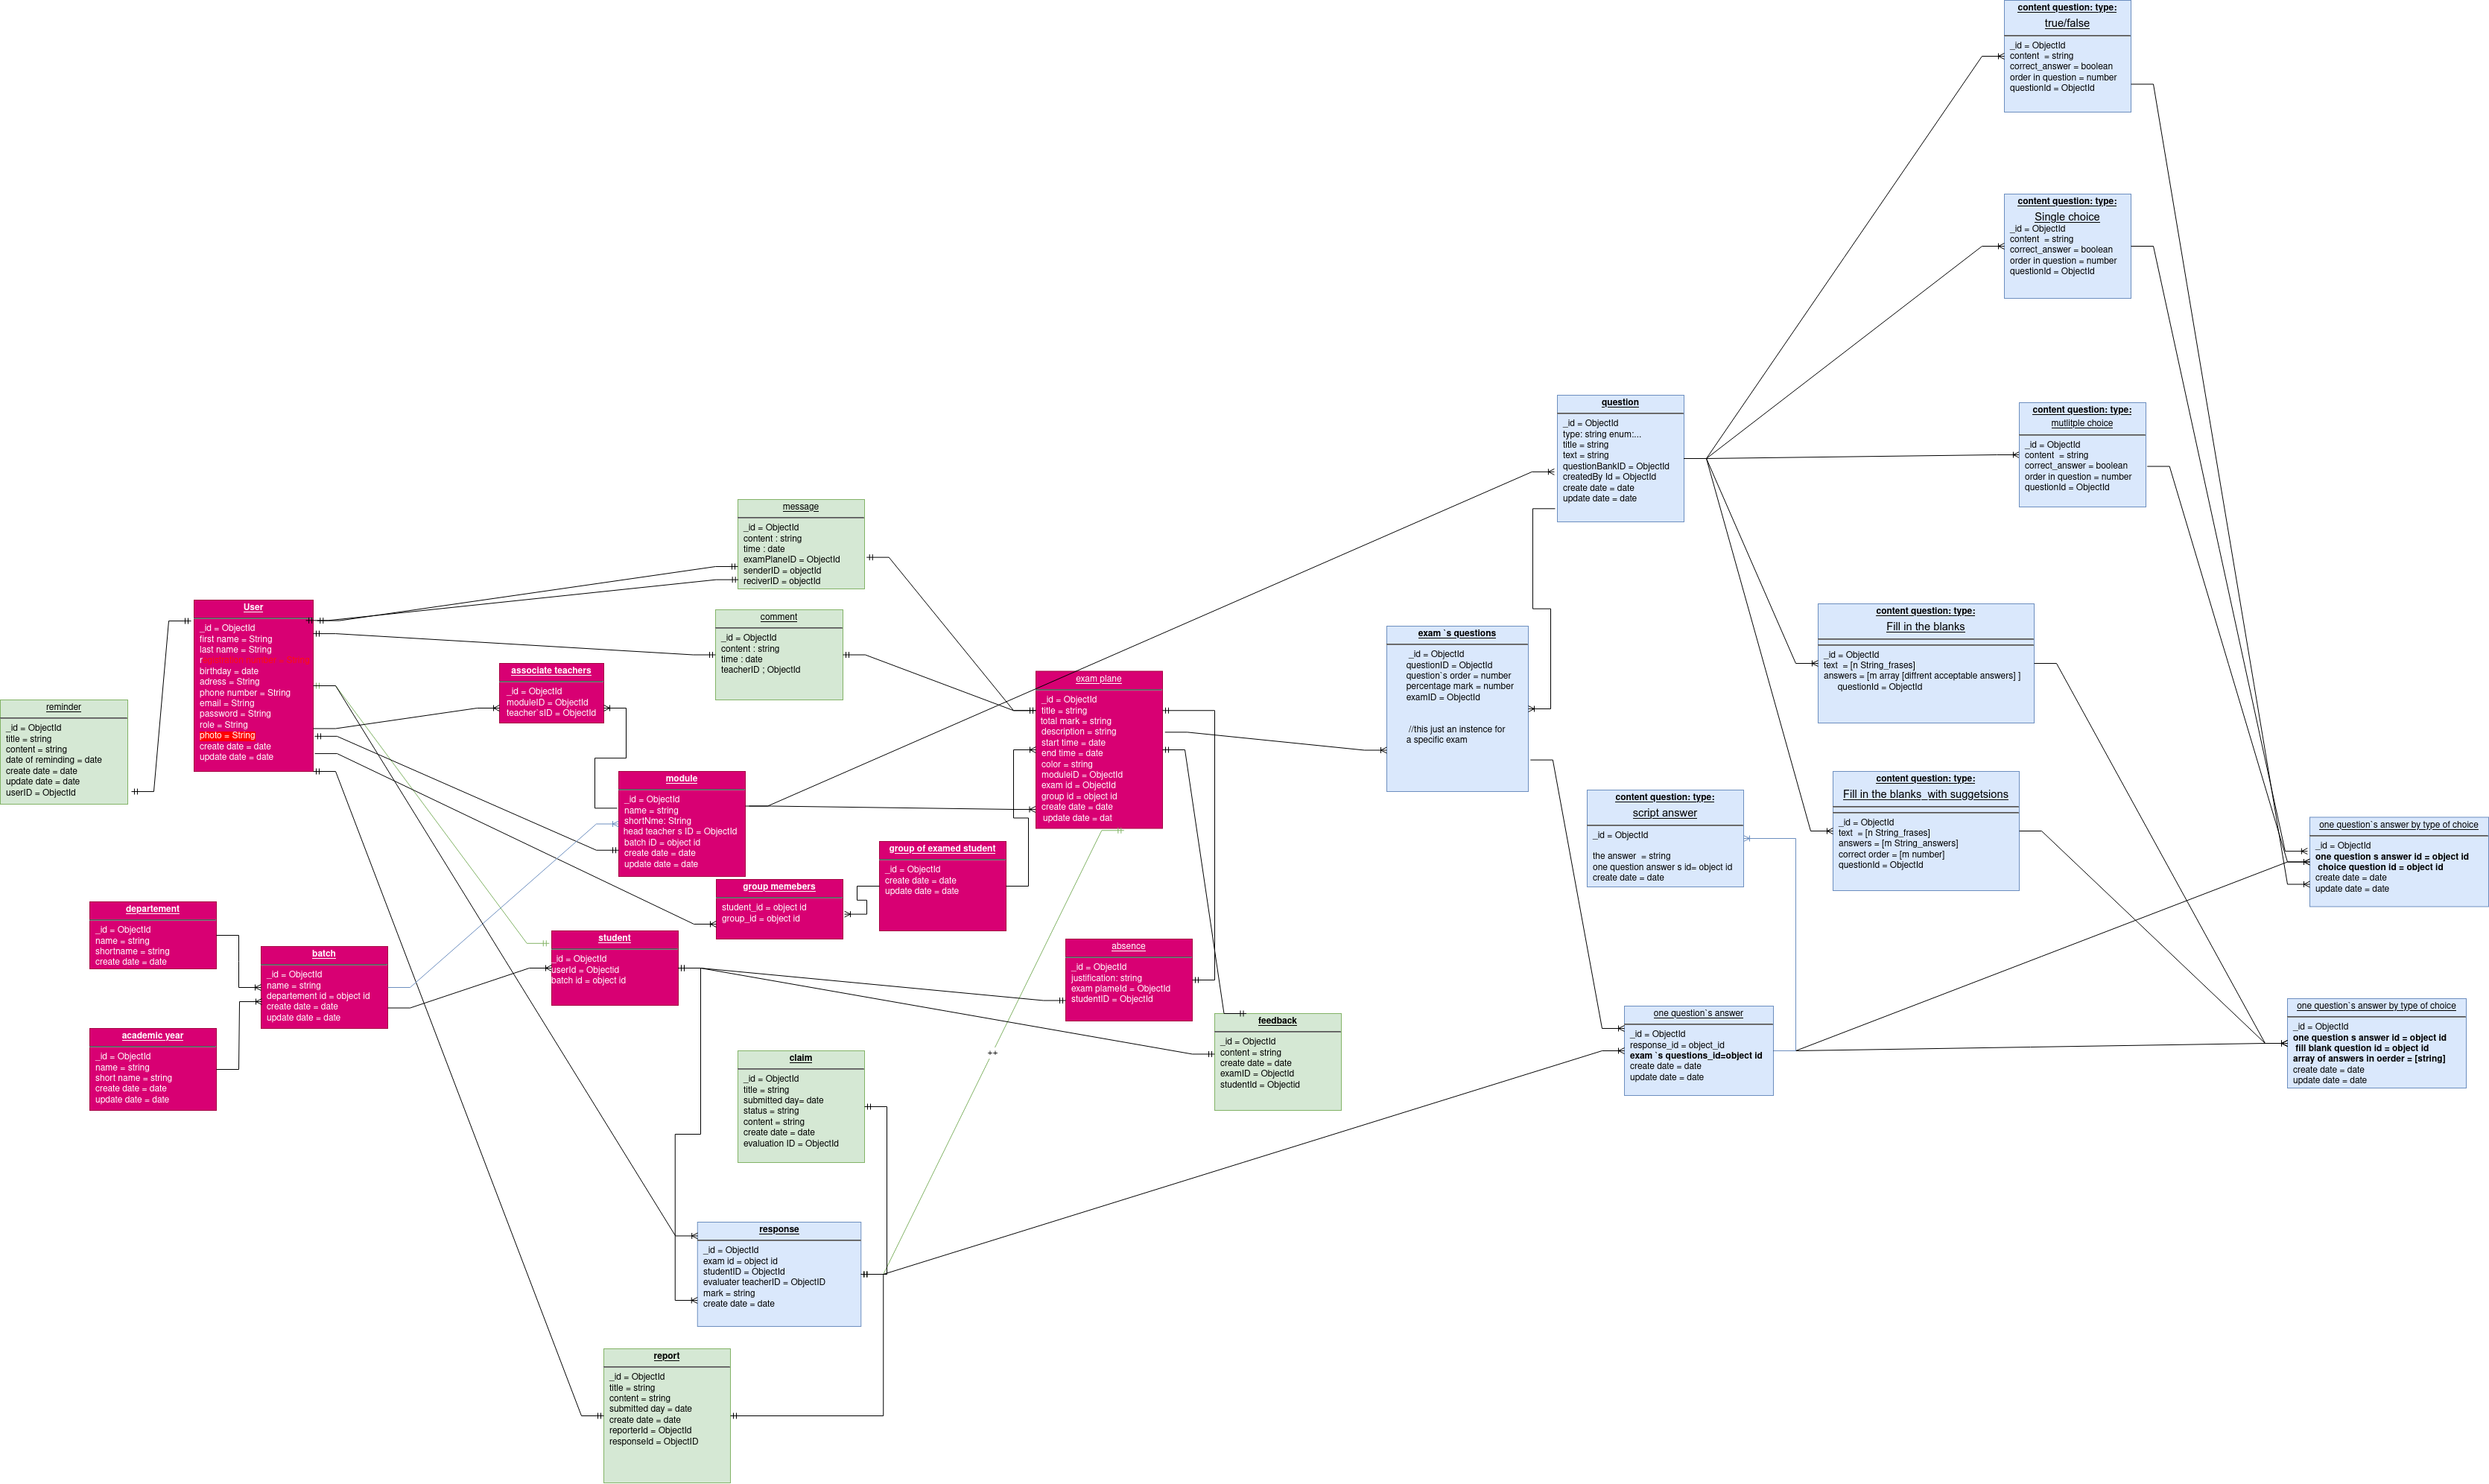
\includegraphics[width=\textwidth]{images/DbSchema}
        \caption{Database schema diagram}
    \end{figure}
    \clearpage
    \raggedright\section{Conclusion}


\end{document}